\documentclass[12pt,a4paper]{article}
\usepackage[utf8]{inputenc}
\usepackage[spanish]{babel}
\usepackage{graphicx}
\usepackage{amsmath}
\usepackage{listings}
\usepackage{xcolor}
\usepackage{hyperref}
\usepackage{geometry}
\usepackage{float}

% Configuración de márgenes
\geometry{
    a4paper,
    top=2.5cm,
    bottom=2.5cm,
    left=3cm,
    right=3cm
}

% Configuración de listings para código Python
\lstset{
    language=Python,
    basicstyle=\ttfamily\small,
    numbers=left,
    numberstyle=\tiny,
    frame=single,
    breaklines=true,
    breakatwhitespace=false,
    showstringspaces=false,
    keywordstyle=\color{blue},
    commentstyle=\color{green!60!black},
    stringstyle=\color{red}
}

\begin{document}

% Portada
\begin{titlepage}
    \begin{center}
        \vspace*{2cm}
        {\LARGE\textbf{Fundamentos de las Comunicaciones Digitales}}\\[1cm]
        {\Large Trabajo Práctico}\\[4cm]
        {\large\textbf{Simulación de Sistemas de Transmisión Digital}}\\[1cm]
        {\large Ejercicio 1: Transmisión en Banda Base}\\
        {\large Ejercicio 2: Transmisión Digital Modulada}\\[4cm]
        {\large\today}\\[2cm]
        {\large\textbf{Autores:}}\\[0.5cm]
        {\large Estrada, Matías Valentin}\\
        {\large Uriarte, Luca Emiliano}
    \end{center}
\end{titlepage}

\tableofcontents
\newpage

\section{Introducción}
Este trabajo práctico implementa simulaciones de sistemas de transmisión digital, abordando dos aspectos fundamentales:
transmisión en banda base y transmisión digital modulada. El código está desarrollado en Python, utilizando bibliotecas
como NumPy para el procesamiento de señales y Matplotlib para la visualización.

\subsection{Parámetros Globales del Sistema}
El programa utiliza varios parámetros globales que afectan a todas las simulaciones:

\begin{lstlisting}[caption=Parámetros globales]
spp = 10000  # Muestras por pulso
A = 1        # Amplitud base de las señales
\end{lstlisting}

Estos parámetros pueden modificarse para:
\begin{itemize}
    \item \texttt{spp}: Aumentar o disminuir la resolución de las señales
    \item \texttt{A}: Cambiar la amplitud base de todas las señales
\end{itemize}

\section{Ejercicio 1: Transmisión en Banda Base}

\subsection{Nivel 1: Simulación Básica}
En este nivel se implementaron simulaciones de formas de onda y densidades espectrales para dos formatos de transmisión.

\subsubsection{Parámetros Configurables}
\begin{lstlisting}[caption=Parámetros del Nivel 1]
# Parámetros generales
A = 1                    # Amplitud de los pulsos
n_bits = 8               # Número de bits a simular
bits = rand_key(n_bits)  # Secuencia aleatoria de bits
\end{lstlisting}

El usuario puede modificar:
\begin{itemize}
    \item \texttt{A}: Amplitud de los pulsos
    \item \texttt{n\_bits}: Longitud de la secuencia a transmitir
    \item \texttt{bits}: Usar \texttt{rand\_key()} para secuencia aleatoria o definir manualmente
\end{itemize}

\subsubsection{Resultados de Ejemplo}
Para una secuencia de 8 bits con los parámetros por defecto, se obtienen las siguientes visualizaciones:

\begin{figure}[H]
    \centering
    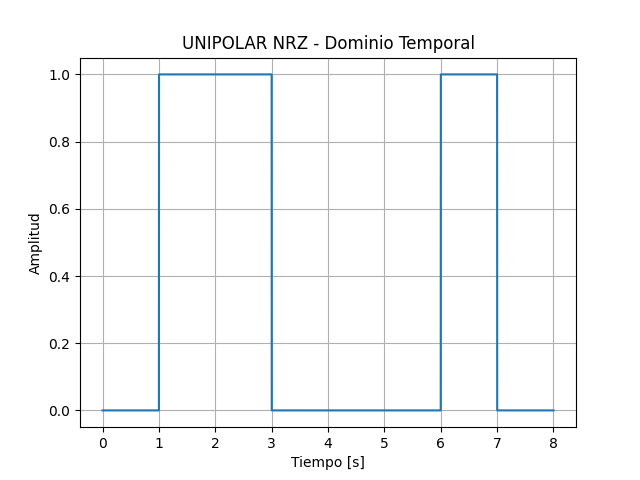
\includegraphics[width=0.8\textwidth]{unrz_time.png}
    \caption{Señal Unipolar NRZ en el dominio temporal}
\end{figure}

\begin{figure}[H]
    \centering
    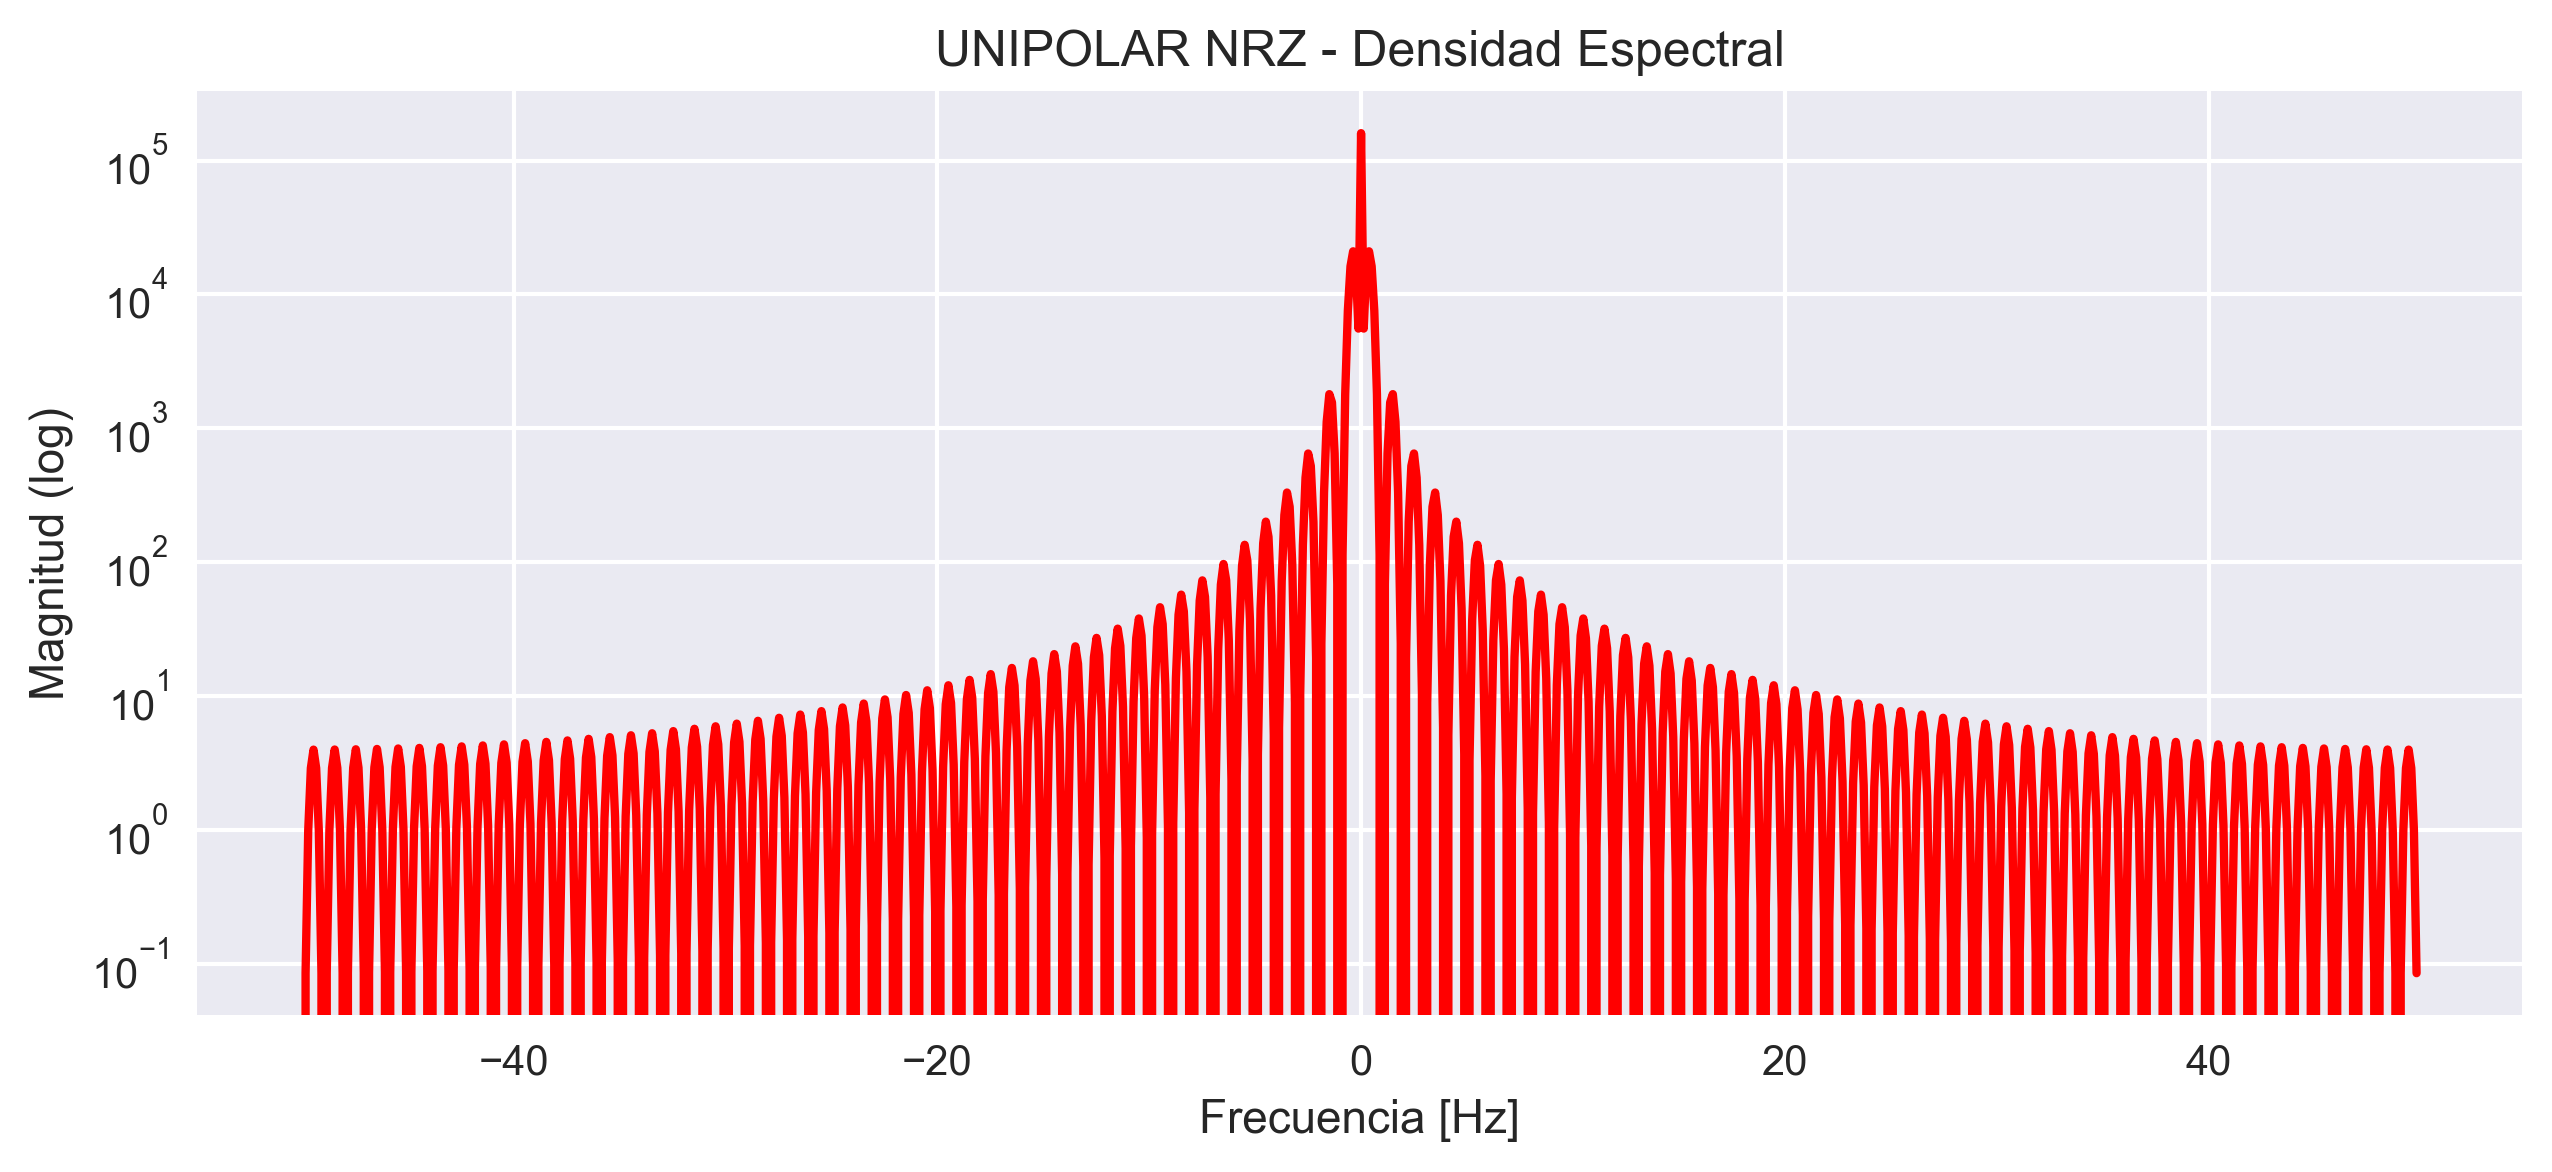
\includegraphics[width=0.8\textwidth]{unrz_freq.png}
    \caption{Densidad espectral de potencia Unipolar NRZ}
\end{figure}

\subsection{Nivel 2: Script Genérico}
El script genérico permite una mayor flexibilidad en la configuración de las simulaciones.

\subsubsection{Parámetros Configurables}
\begin{lstlisting}[caption=Parámetros del Nivel 2]
# Parámetros base
A = 1        # Amplitud
n_bits = 12  # Número de bits
fc = 1000    # Frecuencia de portadora
M = 4        # Orden de modulación
RZ = 1       # Factor de retorno a cero
ret_amp = 0  # Amplitud de retorno
\end{lstlisting}

El usuario puede:
\begin{itemize}
    \item Seleccionar el formato de transmisión:
    \begin{itemize}
        \item unipolarNRZ
        \item polarNRZ
        \item unipolarRZ
        \item polarRZ
        \item manchester
        \item AMI
        \item M-ASK
    \end{itemize}
    \item Elegir el tipo de pulso (rectangular o sinc)
    \item Modificar todos los parámetros mencionados
\end{itemize}

\subsection{Nivel 3: Análisis de Error}
Este nivel implementa el análisis de la tasa de error de bit (BER).

\subsubsection{Parámetros Configurables}
\begin{lstlisting}[caption=Parámetros del Nivel 3]
# Parámetros
A = 1                           # Amplitud
N = 100                        # Bits por simulación
formato = "polarNRZ"           # Formato de transmisión
snr_db_range = np.arange(0, 11, 1)  # Rango de SNR
\end{lstlisting}

El usuario puede modificar:
\begin{itemize}
    \item \texttt{N}: Número de bits para la simulación de error
    \item \texttt{snr\_db\_range}: Rango de valores SNR a simular
    \item \texttt{formato}: Tipo de codificación a analizar
\end{itemize}

\begin{figure}[H]
    \centering
    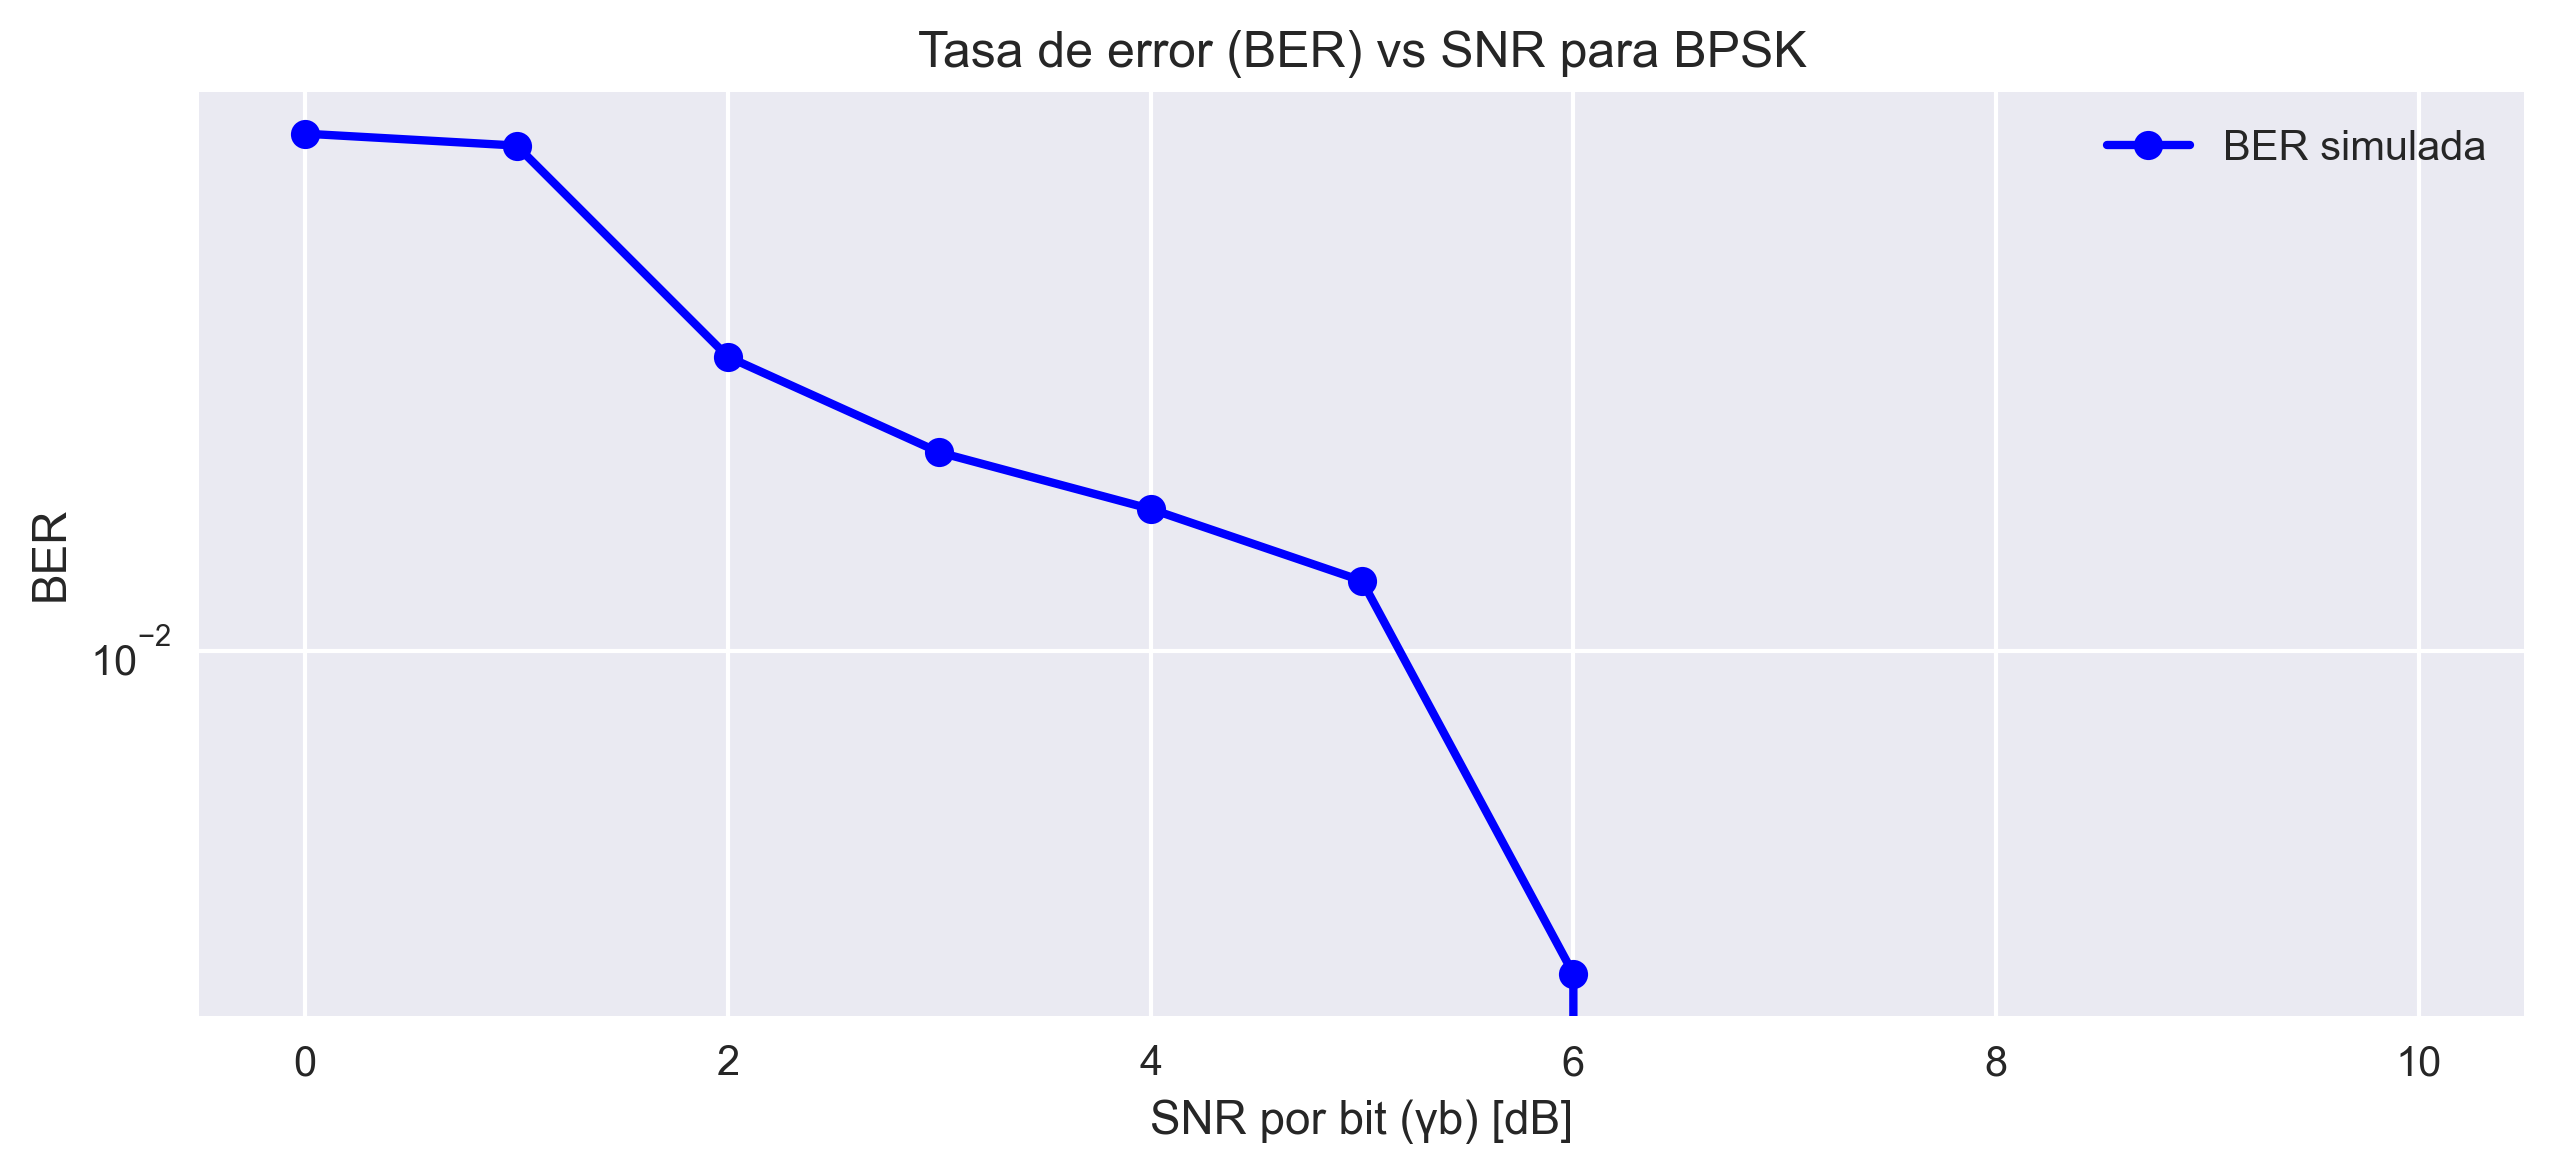
\includegraphics[width=0.8\textwidth]{ber_vs_snr.png}
    \caption{Tasa de error de bit vs SNR para polarNRZ}
\end{figure}

\section{Ejercicio 2: Transmisión Digital Modulada}

\subsection{Nivel 1: Modulaciones Básicas}
Este nivel implementa modulaciones digitales básicas 2-PSK y 8-PSK.

\subsubsection{Parámetros Configurables}
\begin{lstlisting}[caption=Parámetros del Nivel 1]
# Parámetros generales
A = 1                      # Amplitud de la señal
fc = 2000                  # Frecuencia de portadora
n_bits = 10                # Número de bits
\end{lstlisting}

El usuario puede modificar:
\begin{itemize}
    \item \texttt{A}: Amplitud de la señal modulada
    \item \texttt{fc}: Frecuencia de la portadora
    \item \texttt{n\_bits}: Longitud de la secuencia
\end{itemize}

\begin{figure}[H]
    \centering
    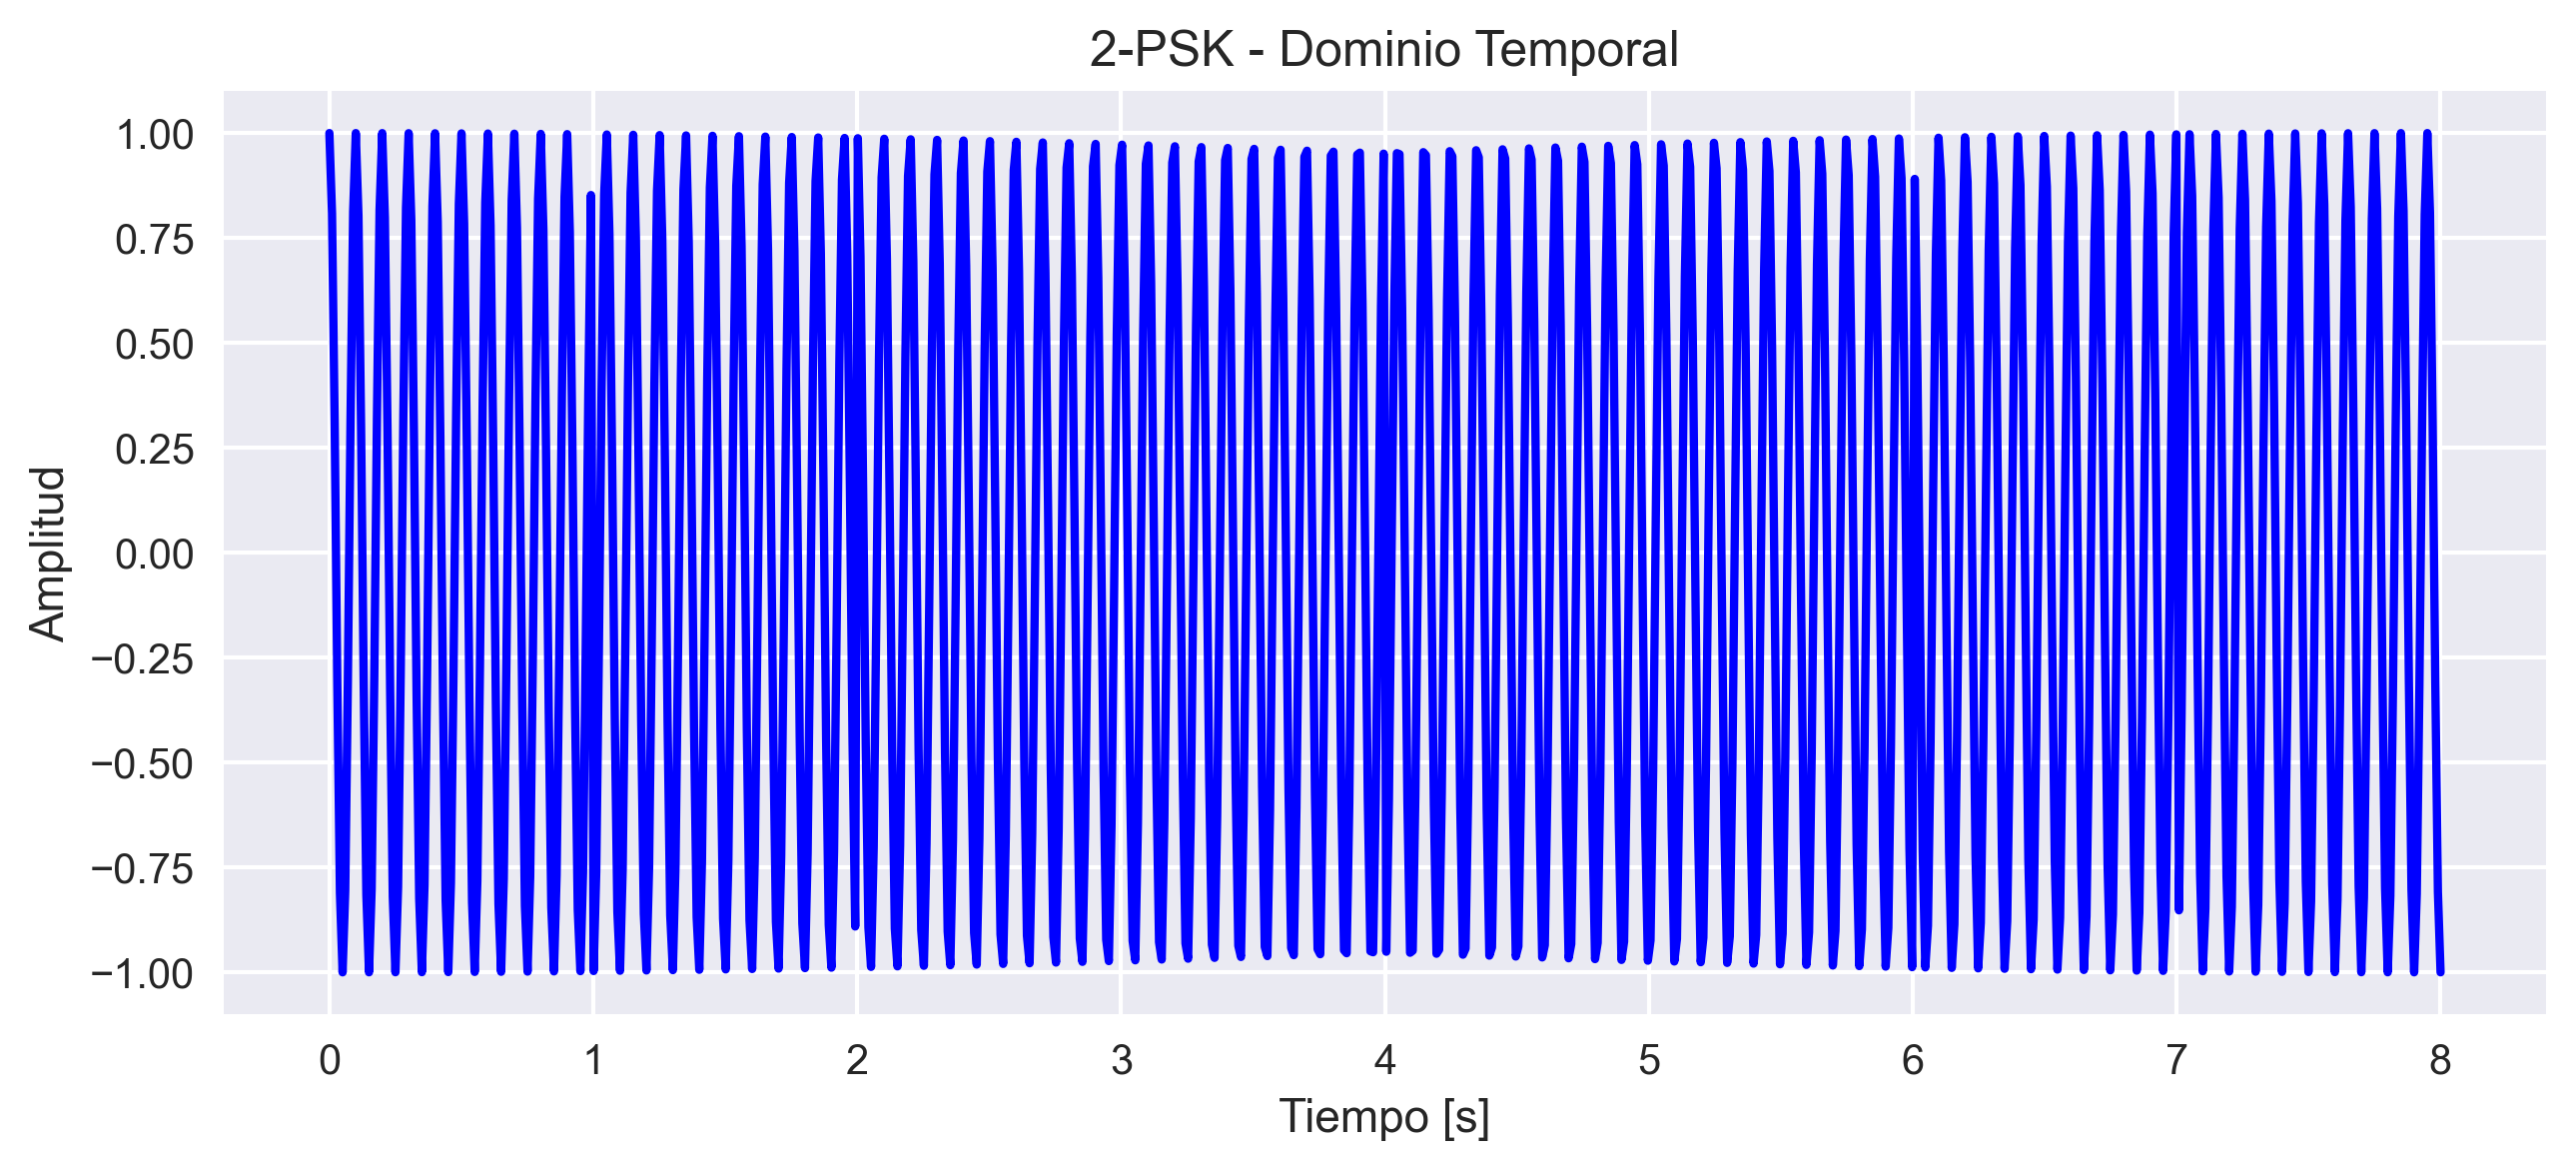
\includegraphics[width=0.8\textwidth]{2psk_time.png}
    \caption{Señal 2-PSK en el dominio temporal}
\end{figure}

\begin{figure}[H]
    \centering
    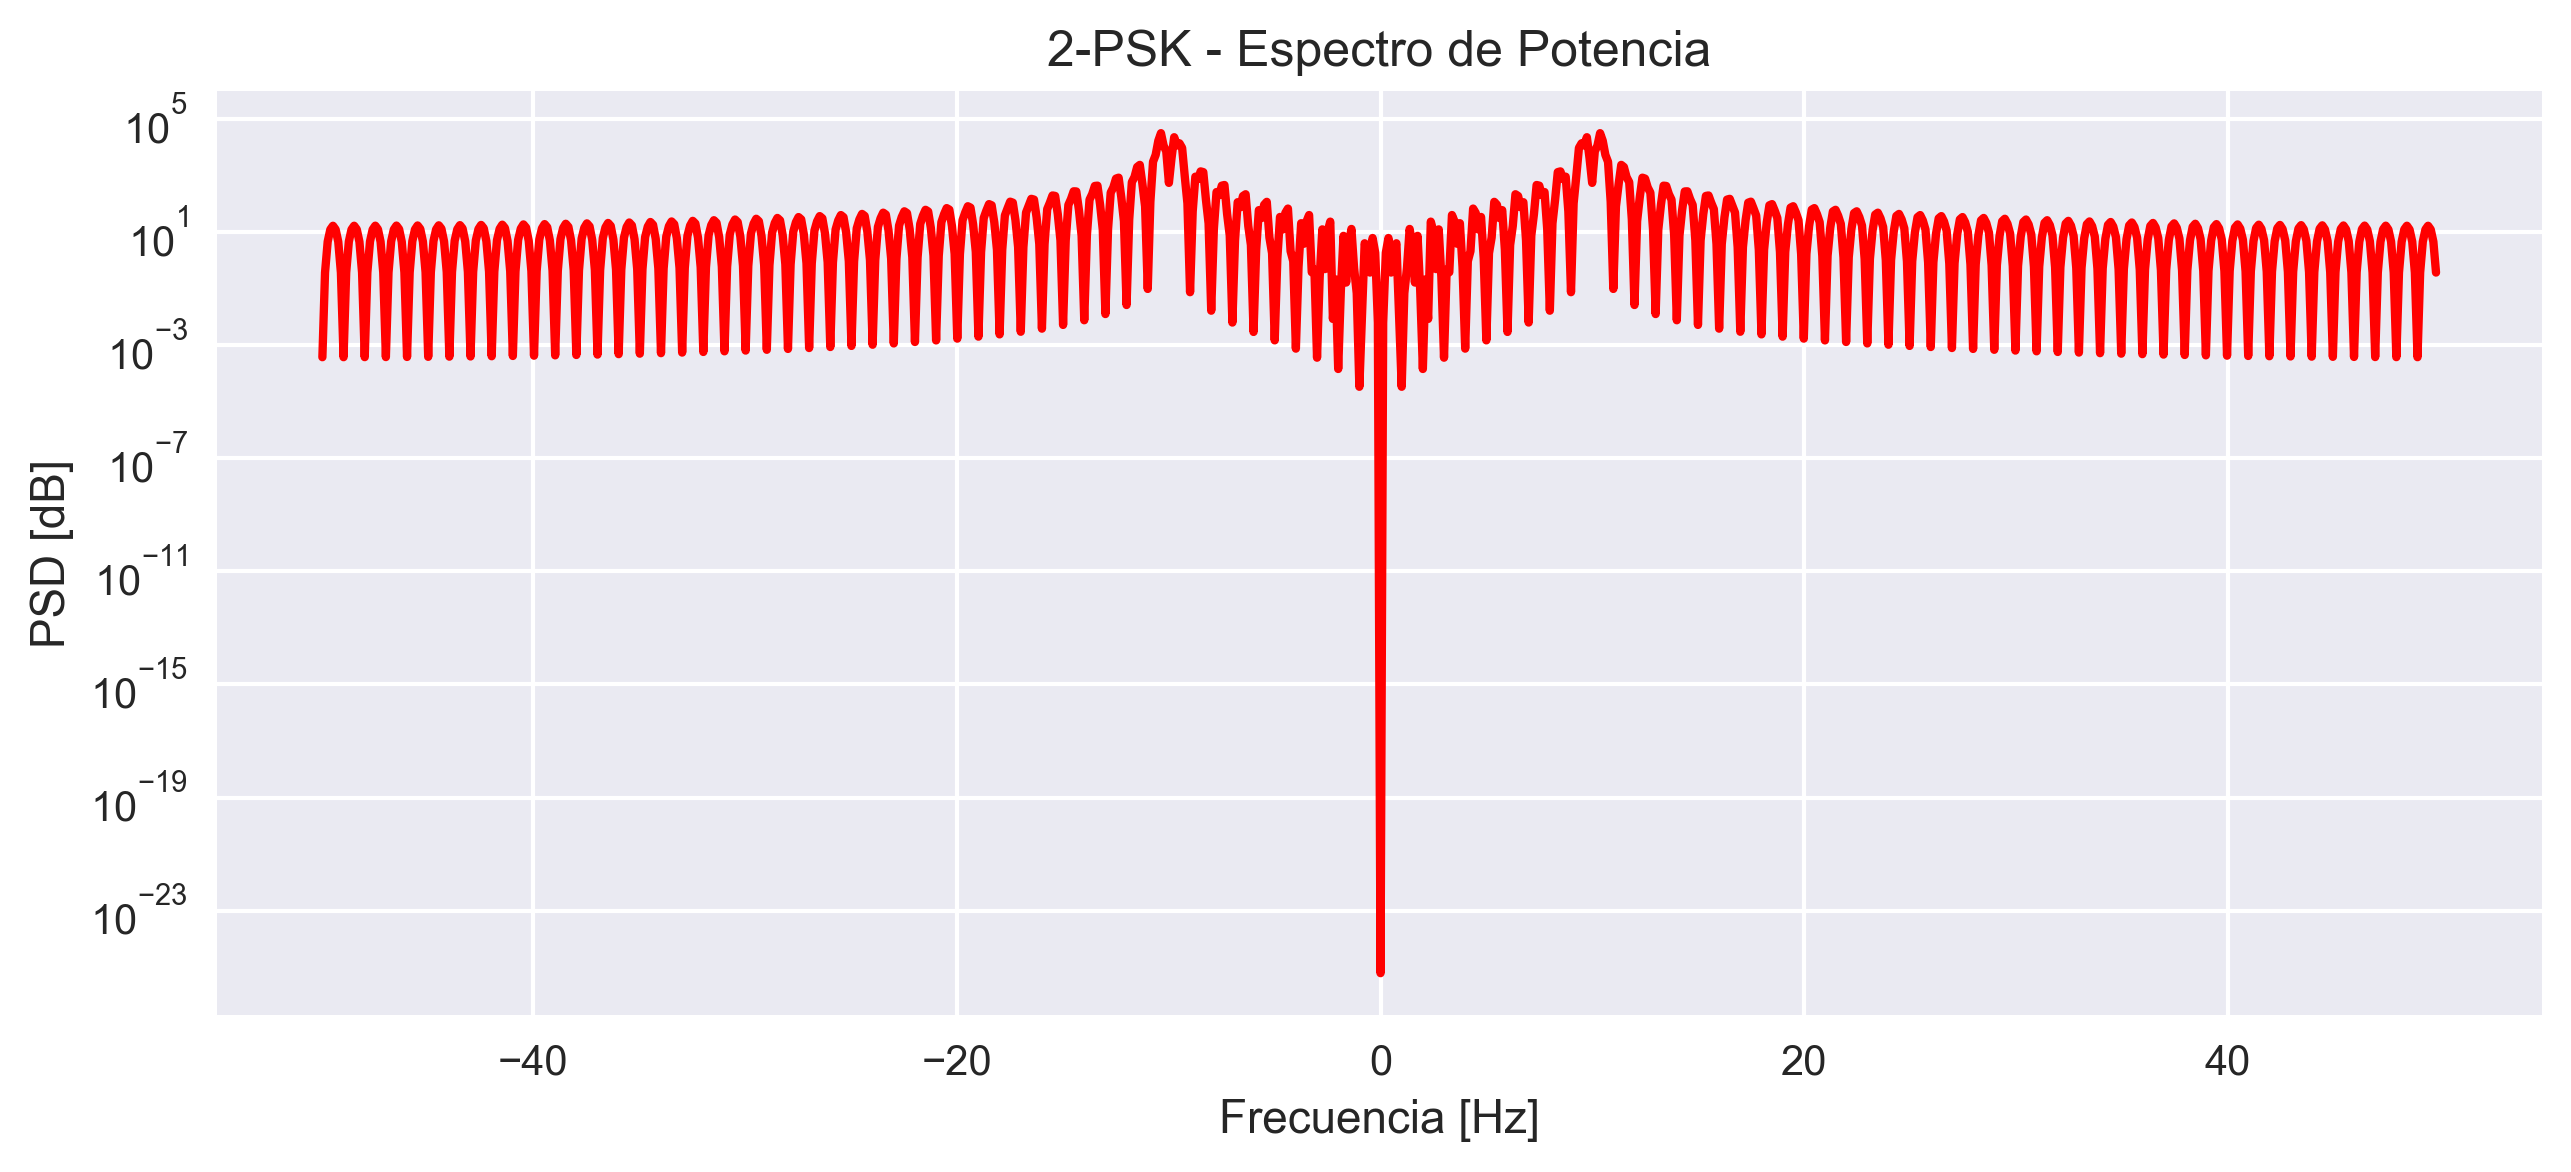
\includegraphics[width=0.8\textwidth]{2psk_freq.png}
    \caption{Espectro de potencia 2-PSK}
\end{figure}

\subsection{Nivel 2: Script Genérico para Modulaciones}
La función genérica permite simular cualquier modulación digital soportada.

\subsubsection{Parámetros de la Función}
\begin{lstlisting}[caption=Parámetros de simulate\_digital\_modulation]
def simulate_digital_modulation(
    modulation_type,  # 'ASK', 'PSK', 'QAM'
    M,               # Orden de modulación (2^n)
    A=1,            # Amplitud
    n_bits=None,    # Número de bits
    fc=1000         # Frecuencia portadora
):
\end{lstlisting}

El usuario puede:
\begin{itemize}
    \item Elegir el tipo de modulación
    \item Configurar el orden de modulación M
    \item Ajustar amplitud y frecuencia portadora
    \item Especificar la longitud de la secuencia
\end{itemize}

\subsection{Nivel 3: Análisis de Tasa de Error}
Este nivel analiza el rendimiento de diferentes esquemas de modulación.

\subsubsection{Parámetros Configurables}
\begin{lstlisting}[caption=Parámetros del análisis de error]
def calculate_symbol_error_rate(
    modulation_type,  # Tipo de modulación
    M,               # Orden de modulación
    n_symbols=1000,  # Símbolos a simular
    snr_db_range=None  # Rango de SNR
):
\end{lstlisting}

El usuario puede modificar:
\begin{itemize}
    \item Tipo y orden de modulación
    \item Número de símbolos para la simulación
    \item Rango de valores SNR a analizar
\end{itemize}

\begin{figure}[H]
    \centering
    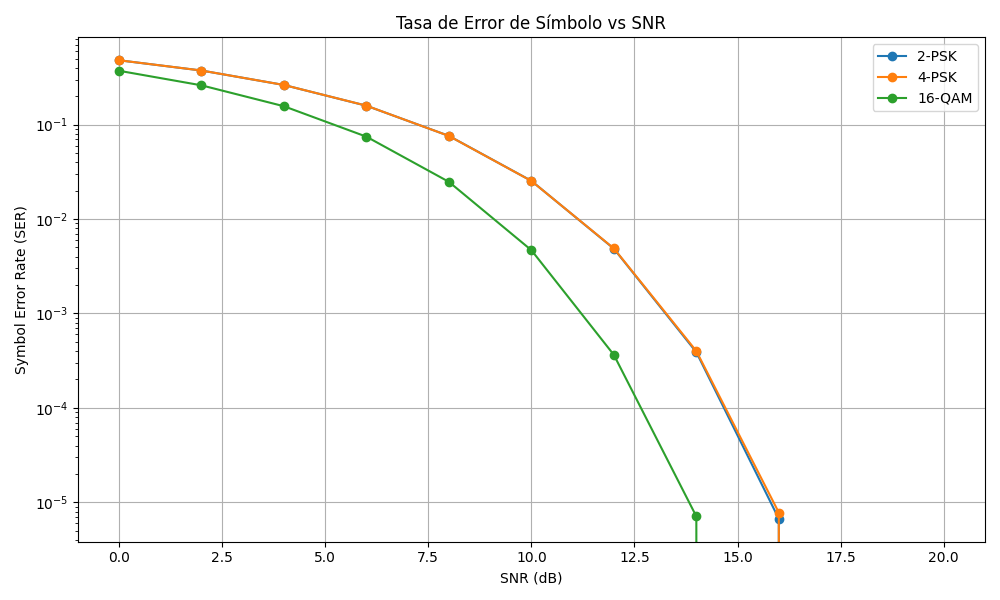
\includegraphics[width=0.8\textwidth]{ser_comparison.png}
    \caption{Comparación de SER para diferentes modulaciones}
\end{figure}

\section{Conclusiones}
El trabajo implementa exitosamente una amplia gama de técnicas de transmisión digital, tanto en banda base como moduladas.
Las simulaciones permiten observar y comparar:
\begin{itemize}
    \item Características espectrales de diferentes formatos de transmisión
    \item Efecto del pulso conformador (rectangular vs sinc)
    \item Compromiso entre eficiencia espectral y robustez al ruido
    \item Rendimiento de diferentes esquemas de modulación
\end{itemize}

\section{Instrucciones de Uso}
Para utilizar el programa:

\begin{enumerate}
    \item Asegurarse de tener instaladas las bibliotecas necesarias:
    \begin{lstlisting}
import numpy as np
import matplotlib.pyplot as plt
from scipy.fft import fft, fftshift
    \end{lstlisting}
    
    \item Ejecutar el script principal \texttt{tp\_fcd.py}
    \item Para modificar parámetros:
    \begin{itemize}
        \item Editar las variables globales al inicio del archivo
        \item Modificar los parámetros específicos en cada sección
        \item Ajustar los parámetros de visualización según necesidad
    \end{itemize}
    \item Los resultados se mostrarán automáticamente en gráficos
\end{enumerate}

\end{document} 